\documentclass{sciposter}
\usepackage{lipsum}
\usepackage{epsfig}
\usepackage{amsmath}
\usepackage{amssymb}
\usepackage{multicol}
\usepackage{graphicx,url}
\usepackage[spanish]{babel}   
\usepackage[utf8]{inputenc}
%\usepackage{fancybullets}
\newtheorem{Def}{Definition}


\title{Reconocimiento de actividades humanas con un enfoque colaborativo}
%Título do projeto

\author{Alberto Gimenez, Santiago A. Yegros Z, Joaquín Lima}
%nome dos autores

\institute 
{Facultad Politécnica - Universidad Nacional de Asunción \\
  San Lorenzo, Paraguay}
%Nome e endereço da Instituição

\email{{albergimenez@gmail.com, santiago.yegros@gmail.com, joaquin.lima@pol.una.py}}
% Onde você coloca os emails dos integrantes


%\date is unused by the current \maketitle

\rightlogo[1]{logo}
\leftlogo[1]{logo.jpg}
% Exibe os logos (direita e esquerda) 
% Procure usar arquivos png ou jpg, e de preferencia mantenha na mesma pasta do .tex
%%%%%%%%%%%%%%%%%%%%%%%%%%%%%%%%%%%%%%%%%%%%%%%%%%%%%%%%%%%%%%%%%%%%%%%%%%%%%%%%
%%% Begin of Document



\begin{document}
%define conference poster is presented at (appears as footer)

\conference{Diciembre 2017}

%\LEFTSIDEfootlogo  
% Uncomment to put footer logo on left side, and 
% conference name on right side of footer

% Some examples of caption control (remove % to check result)

%\renewcommand{\algorithmname}{Algoritme} % for Dutch

%\renewcommand{\mastercapstartstyle}[1]{\textit{\textbf{#1}}}
%\renewcommand{\algcapstartstyle}[1]{\textsc{\textbf{#1}}}
%\renewcommand{\algcapbodystyle}{\bfseries}
%\renewcommand{\thealgorithm}{\Roman{algorithm}}

\maketitle

%%% Begin of Multicols-Enviroment
\begin{multicols}{3}

%%% Abstract
\begin{abstract}
El reconocimiento de actividades humanas (HAR, \textit{Human Activity Recognition}) es un tópico ampliamente cubierto en la última década por su relevancia en aplicaciones dependientes del contexto. Dada la capacidad de los teléfonos móviles inteligentes de recopilar datos del entorno e incorporar algoritmos de razonamiento, estos se convierten en una poderosa plataforma para construir aplicaciones con información de contexto. En este trabajo, se propone un sistema de código abierto denominado \textit{HARDroid} específicamente diseñado para detectar actividades humanas básicas para la plataforma \textit{Android}. Adicionalmente, se aporta un modelo de mejora continua del clasificador de actividades por medio de la colaboración de datos recopilados en terreno. Finalmente, se presenta una evaluación que compara el clasificador entrenado inicialmente y el clasificador colaborativo logrando mejora en exhaustividad del 91,34\%, una precisión del 92,04\% y una exactitud del 97,23\%. 
\\
\textbf{Palabras Claves}
Sensores, Aprendizaje Automático, Aplicación de Contexto, Teléfonos móviles, Colaboración .
\end{abstract}

%%% Introduction
\section{Introducción}

HAR es un área de investigación en constante desarrollo que abarca el diseño de algoritmos para recolectar datos ambiguos capturados del entorno de individuos para proporcionar información contextual durante su interacción [2]. Uno de los contextos más relevantes es reconocer las actividades humanas que consisten en las caminar, correr o las posturas como estar pie o sentado, todo esto a través de algún sensor disponible.

A medida que el uso de los teléfonos móviles inteligentes fue masificado, el desarrollo de las aplicaciones basadas en HAR han sido propicias a fin de mejorar la interacción con los usuarios. El uso de información contextual es para diversos fines y tipos de sistemas inteligentes, por ejemplo, en medicina, cuidado personal, entretenimiento o uso militar \cite{LaraLabrador2013}.

Este trabajo consiste en la aplicación de HAR en teléfonos inteligentes para obtener ude uso libre y de fácil integración. Además, se evalúa la mejora continua del clasificador de actividades por medio de la inclusión datos generados a partir del uso del mismo.

\newcommand{\imsize}{0.45\columnwidth}

\section{Metodología HAR}

Un sistema HAR es similar a otras aplicaciones de aprendizaje automático donde el proceso de reconocimiento se divide en dos etapas bien conocidas como: entrenamiento y evaluación. En la Figura \ref{fig:harsystem2} se resume las fases comunes de estas dos etapas \cite{LaraLabrador2013}. El entrenamiento requiere inicialmente un conjunto de datos recolectados con los atributos medidos de los individuos al realizar cada actividad. La señal se divide luego en ventanas para la extracción de muestras y filtrando para obtener así información relevante de las señales en bruto.

Luego, se utilizan métodos de aprendizaje automático para generar un clasificador de actividades a partir del conjunto de datos de entrenamiento con los valores característicos calculados.

\textbf{Recolección}

El primer paso en el proceso recolectar las señales de los sensores que continuamente monitorean a los usuarios; los sensores pueden estar unidos al cuerpo o ser transportados ya que comúnmente están integrados en teléfonos inteligentes, en relojes o lentes inteligentes. Las señales de los sensores se pueden clasificar según el movimiento, la posición, el entorno y la fisiología \cite{LaraLabrador2013}.

\textbf{Procesamiento}

El siguiente paso es el procesamiento de las señales obtenidas y extraer las características relevantes. El clasificador de actividades se construye a partir de un conjunto de muestras utilizando métodos de aprendizaje automático durante el entrenamiento \cite{reyes}. El procesamiento incluye tres tareas distintas realizadas automáticamente en ambas etapas del proceso HAR, además se realiza una tarea manual durante la etapa de entrenamiento.
\begin{itemize}
	\item Etiquetado
	\item Filtro de Señal
	\item Muestreo
	\item Extracción de muestras
\end{itemize}

\begin{figure}
	\centering
	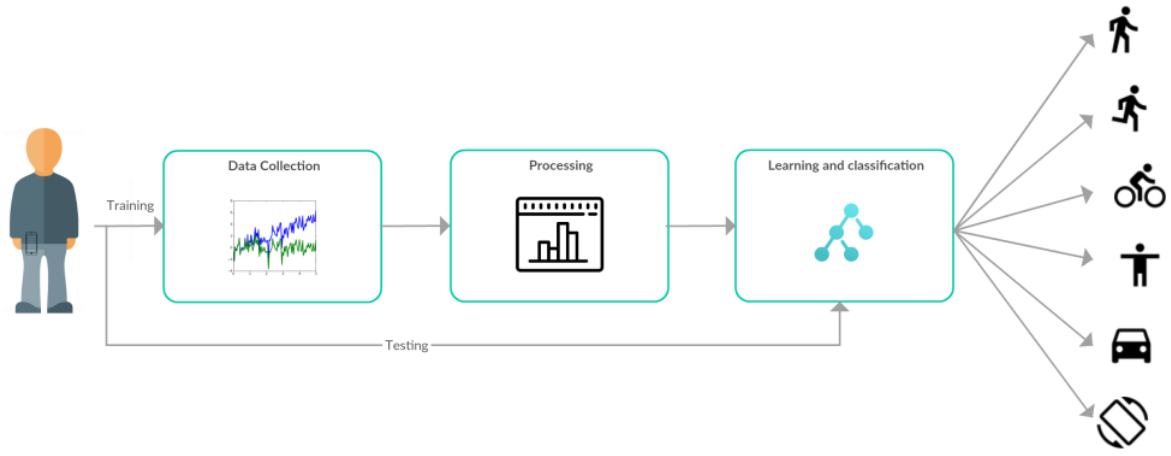
\includegraphics[width=0.7\linewidth]{../capitulo-2/graphics/harsystem2}
	\caption{Metodología HAR}
	\label{fig:harsystem2}
\end{figure}

Las señales procesadas corresponden al atributo de aceleración. Con el fin de minimizar los efectos causados por los cambios de orientación, se calcula la magnitud del acelerómetro, a partir de las dimensiones $x$, $y$, $z$. Esta elección es porque la magnitud es menos sensible a los cambios de orientación. 

\textbf{Aprendizaje y Clasificación}

Un sistema HAR requiere de un algoritmo para extraer información de los datos. El objetivo es clasificar datos desconocidos. Hay muchos algoritmos de aprendizaje, como \textit{Decision Trees}, \textit{SVM}, \textit{Neural Networks}, entre otros. Este trabajo se utiliza un clasificador construido con el algoritmo C4.5 basado en árbol de decisión cuya implementación depende de Java J48 \cite{Frank2016b}.


\section{HARDroid}
HARDroid es un sistema que clasifica las actividades humanas en teléfonos inteligentes basados en Android. El sistema tiene dos componentes: una interfaz de programación de aplicaciones (API) y un servicio en segundo plano que realiza las tareas clave independiente que implementa algoritmos de procesamiento de muestras y reconocimiento. El diseño desacoplado logra un sistema HAR extensible. que permite una fácil evolución y mantenimiento sin afectar a las aplicaciones dependientes. El servicio está pensado como un servicio de utilidad capaz de actualizar el clasificador de actividades de forma dinámica. La Figura \ref{fig:hardroid} muestra el esquema de integración de servicios HARDroid para aplicaciones distribuidas.

\begin{figure}
	\centering
	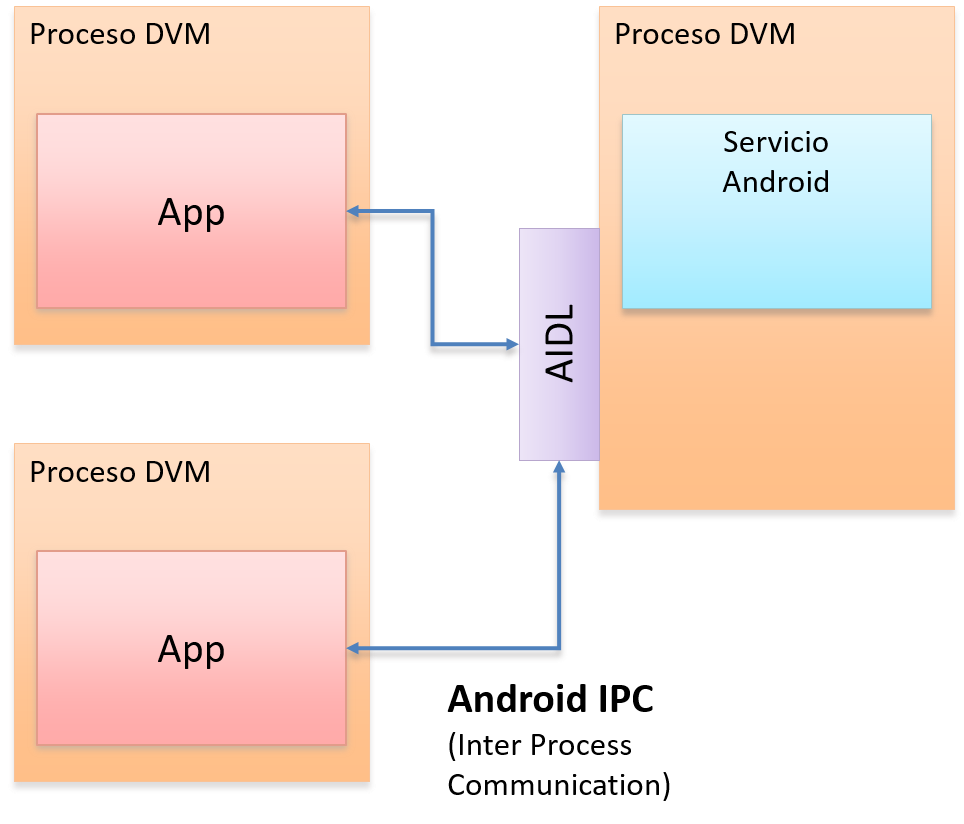
\includegraphics[width=0.7\linewidth]{../capitulo-5/graphics/hardroid_func}
	\caption{Integración de servicio HARDroid.}
	\label{fig:hardroid}
\end{figure}

El clasificador dinámico se actualiza frecuentemente por medio de la colaboración y se descarga de Internet de forma segura empaquetado en un JAR \cite{Falsina2014}.

Para verificar el funcionamiento del servicio HARDroid y evaluar los resultados de reconocimiento, se creó la aplicación ActivitySurvey para probar la integración y encuestar a usuarios reales. Las respuestas a las encuestas son utilizadas para mejorar el clasificador al sincronizar los datos con un servicio web REST llamado Backend C4.5. En la Figura \ref{fig:arq-hardroid} se muestra la arquitectura del proyecto.

\begin{figure}
	\centering
	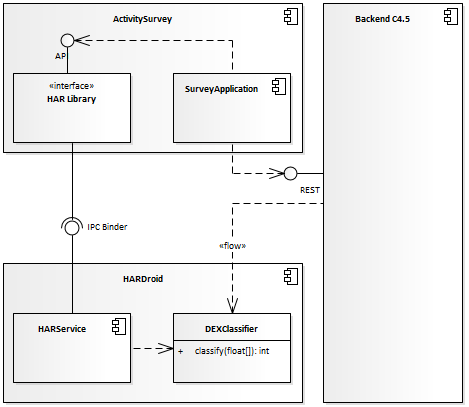
\includegraphics[width=0.7\linewidth]{../capitulo-5/graphics/arqui_general}
	\caption{Arquitectura del Proyecto.}
	\label{fig:arq-hardroid}
\end{figure}

\section{Resultados}

\textbf{Datos Experimentales}

Los datos experimentales se obtuvieron de un grupo de voluntarios de entre 20 y 38 años. El procedimiento de captura de datos se hizo con el uso del teléfono inteligente en el bolsillo mientras se realizaba una actividad física en un período de 2 a 15 minutos con una aplicación para el etiquetado de datos. Se recogieron un total de 6.904.165 medidas de 7 teléfonos diferentes que como resultado obtuvieron 12.012 conjuntos de características.

\textbf{Clasificador Inicial}

Se construyo un clasificador con el algoritmo C4.5 con la implementación en Java J48 utilizando WEKA \cite{Frank2016b}. El clasificador es una clase Java ejecutable en Android. Además, la evaluación de la clasificación de los datos de entrenamiento se resume en precisión de 91,74\% y exhaustividad del 91,09\%.

\textbf{Verificación}

La evaluación del clasificador HARDroid se realizó mediante ejercicios guiados donde cada actividad física se realizó durante un período de 10 a 20 minutos usando ActivitySurvey. Este consulta la actividad humana producida a intervalos regulares y se registra la información de la actividad detectada y actividad sugerida por el usuario.

En el Cuadro 1 muestra el recuento de actividades detectadas exitosas y no exitosas en proporción al número total de detecciones recopiladas durante las sesiones de la encuesta.

\begin{table}[!tbph]
\begin{centering}
	\begin{tabular}{|c|c|c|c|}
		\hline 
		\textbf{Actividad} & \textbf{Error} & \textbf{Éxito} & \textbf{Porcentaje} \\ 
		\hline 
		WALKING & 13 & 151 & 92,07\% \\ 
		\hline 
		RUNNING & 13 & 83 & 86,46\% \\ 
		\hline 
		STILL & 8 & 140 & 94,59\% \\ 
		\hline 
		ON\_BICYCLE & 12 & 59 & 83,10\% \\ 
		\hline 
		IN\_VEHICLE & 11 & 83 & 88,30\% \\ 
		\hline 
	\end{tabular} 
\par\end{centering}
\caption{Actividades Detectadas}
\end{table}

Con esto se puede verificar que el clasificador una alta tasa de éxito en la mayoría de las actividades de acuerdo con un promedio de 88,8\%.

\textbf{Clasificador Colaborativo}

Con la información recopilada por colaboración y combinada con datos iniciales el resultado es un clasificador de actividades generado con instancias correctamente clasificadas resultan en una precisión del 92,04\%, exhaustividad del 91,34\% y aumento de características a 12.578. Por lo tanto, el clasificador colaborativo es una mejora sobre el modelo clasificador inicial por medio de la retroalimentación.

\section{Conclusión}

En este trabajo, un sistema HAR en Android de código abierto es aportado y es reutilizable para reconocer las actividades humanas comunes. Además, el clasificador permite la mejora iterativa de su rendimiento a través de un esquema de colaboración. Las pruebas de evaluación tienen resultados alentadores con una alta tasa de éxito del 92\% y la posibilidad de que el modelo se pueda mejorar con un esfuerzo de colaboración.
 
%%% References

%% Note: use of BibTeX als works!!

\bibliographystyle{plain}
\begin{thebibliography}{1}

\bibitem{LaraLabrador2013}
Oscar D.Lara and Miguel A. Labrador. 2013.
\newblock A Survey on Human Activity Recognition using Wearable Sensors
\newblock In \textit{IEEE Communications Surveys Tutorials} 15, no. 3, 1192-1209.

\bibitem{Falsina2014}
Luca Falsina. Grab’n Run. 2014.
\newblock Retrieved November 20, 2016 from
\newblock http://grab-n-run.readthedocs.io/en/latest/index.html.

\bibitem{Frank2016b}
Eibe Frank. J48 Implementation.
\newblock 2017. Retrieved March 6, 2017 from
\newblock http://weka.sourceforge.net/doc.stable/weka/classifiers/
\newblock trees/J48.html.

\bibitem{reyes}
Jorge Luis Reyes Ortiz. 2015. 
\newblock \textit{Smartphone-Based Human Activity Recognition}
\newblock Springer Theses. Springer International Publishing, Cham. 
\newblock http://dx.doi.org/10.1007/978-3-319-14274-6.

\end{thebibliography}

\end{multicols}

\end{document}